%%%%%%%%%%%%%%%%%%%%%%%%%%%%%%%%%%%%%%%%%
% Beamer Presentation

%
%%%%%%%%%%%%%%%%%%%%%%%%%%%%%%%%%%%%%%%%%


\documentclass[xcolor=rgb]{beamer}

\mode<presentation> {

% The Beamer class comes with a number of default slide themes
% which change the colors and layouts of slides. Below this is a list
% of all the themes, uncomment each in turn to see what they look like.


\usetheme{AnnArbor}


%\usecolortheme{albatross}
%\usecolortheme{beaver}
%\usecolortheme{beetle}
%\usecolortheme{crane}
%\usecolortheme{dolphin}
%\usecolortheme{dove}
%\usecolortheme{fly}
%\usecolortheme{lily}
%\usecolortheme{orchid}
%\usecolortheme{rose}
%\usecolortheme{seagull}
%\usecolortheme{seahorse}
%\usecolortheme{whale}
%\usecolortheme{wolverine}


}

\usepackage{graphicx} % Allows including images
\usepackage{booktabs} % Allows the use of \toprule, \midrule and \bottomrule in tables
\usepackage{caption}
\usepackage{ragged2e} 
\usepackage{multirow}
\usepackage[font=small]{caption}
%\usepackage{cctbase, ccmap, CCTfntef}
\usepackage{wallpaper}
\usepackage{float}

\usepackage{multirow} %by me
\usepackage{color,soul}
\usepackage{lipsum}
\usepackage{tikz} 
\usepackage[export]{adjustbox}
\usepackage{xcolor}
\usepackage{listings}
\usepackage{minted}


%
%----------------------------------------------------------------------------------------
%	TITLE PAGE
%----------------------------------------------------------------------------------------

\title[\textbf{Presentation G4}]{\textbf{GEANT4 for GEometry ANd Tracking}} % The short title appears at the bottom of every slide, the full title is only on the title page

\author{Andreicovici Iulian Florin} % Your name
\institute[UPB] % Your institution as it will appear on the bottom of every slide, may be shorthand to save space
{
Student\\ \textbf{FACULTATEA DE ȘTIINȚE APLICATE (FSA)}\\ \textit{Specializarea}\textendash \textit{IF}\\ 
%%\\Visiting Student, West Virginia University Institute of Technology (WVU Tech) \\ % Your institution for the title page
\medskip
 % Your email address
\textit{\textbf{O prezentare introductivă.\\}}
%\normalsize\textit{Tuesday, March 28, 2017\\IEEE West Virginia Section}
}
\titlegraphic{
\includegraphics[scale = 0.2]{Sim.png} 
\includegraphics[scale = 0.3]{Figures/LOGO/LOGO.png}}
\date[1 August]{01.08.2022} 

% Date, can be changed to a custom date

   \begin{document}

%start
%%%%%%%%%%%%%%%%%%%%%%%%%%%%%%%%%%%%%%%%%%%%%%%%%%%%%%%%%%%%%%%%%%%%%%%%%%%%%

\begin{frame}
\titlepage % Print the title page as the first slide

\end{frame}

%capitol
\begin{frame}
\frametitle{Overview... G4} % Table of contents slide, comment this block out to remove it

\tableofcontents % Throughout your presentation, if you choose to use \section{} and \subsection{} commands, these will automatically be printed on this slide as an overview of your presentation

%logo first

\begin{tikzpicture}[overlay, remember picture]
 \node[anchor=center, 
      xshift=3cm, 
      yshift=1.8cm] 
     at (current page.center)
     {
\includegraphics[width=4.5cm,height=1.5cm]{G4Logo.png}}; 
 \end{tikzpicture}

%image 2 - project
 \begin{tikzpicture}[overlay, remember picture]
 \node[anchor=center, 
      xshift=3cm, 
      yshift=0cm] 
     at (current page.center)
     {
\includegraphics[scale = 0.2]{Project_images/Project.png}}; 
 \end{tikzpicture}

%image 3 - CONCLUSION
 \begin{tikzpicture}[overlay, remember picture]
 \node[anchor=center, 
      xshift=3cm, 
      yshift=-1.5cm] 
     at (current page.center)
     {
\includegraphics[scale = 0.3]{Project_images/Conclusion.png}}; 
 \end{tikzpicture}

%image 4 - 
 \begin{tikzpicture}[overlay, remember picture]
 \node[anchor=center, 
      xshift=-3cm, 
      yshift=-3cm] 
     at (current page.center)
     {
\includegraphics[scale = 0.3]{Project_images/Attention.png}}; 
 \end{tikzpicture}

\end{frame}




%----------------------------------------------------------------------------------------
%	PRESENTATION SLIDES names
%----------------------------------------------------------------------------------------
	
 %Section1
 %------------------------------------------------
	\section{Scurtă introducere in G4.} % Sections can be created in order to organize your presentation into discrete blocks, all sections and subsections are automatically printed in the table of contents as an overview of the talk
	%------------------------------------------------
	



%\subsection{} % A subsection can be created just before a set of slides with a common theme to further break down your presentation into chunks

%part1
\subsection{Câteva cuvinte "lămuritoare"}


%frame1
\begin{frame} 
 \frametitle{\textbf{Motivatie pentru motivatie...}} 

%image 1- CERN Logo
\begin{tikzpicture}[overlay, remember picture]
\node[anchor=center, 
      xshift=4cm, 
      yshift=1cm] 
     at (current page.center)
     {
\includegraphics[scale=0.3]{Project_images/Detector.png}}; 
\end{tikzpicture}

%GEANT4 Present(imag2) C++ fir
\begin{tikzpicture}[overlay, remember picture]
\node[anchor=center, 
      xshift=-4cm, 
      yshift=1cm] 
     at (current page.center) 
     {
\includegraphics[scale = 0.15]{Project_images/c++.png}}; 
\end{tikzpicture}

%GEANT4 Present(imag2) Cern
\begin{tikzpicture}[overlay, remember picture]
\node[anchor=center, 
      xshift=0cm, 
      yshift=1cm] 
     at (current page.center) 
     {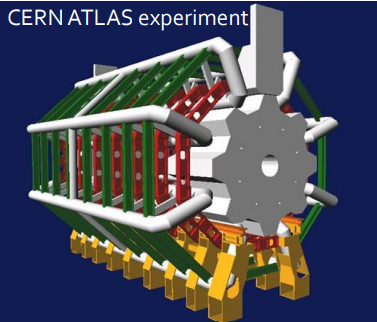
\includegraphics[scale = 0.4]{Project_images/Cern.png}}; 
\end{tikzpicture}


%text
 \vspace*{2.0cm} %pozitionare relativ la head

 \textbf{...De ce GEANT4?} 
\begin{enumerate}
  \item \textit{-Este o platformă destinată simulării interacțiunii particulelor cu materia.}
  \item \textit{-Se bazează integral pe limbajul C++(paradigma OOP).}
  \item \textit{-Are numeroase aplicații în fizica energiilor înalte cât și în fizica nucleară.}
\end{enumerate}
\end{frame}



%%%%%%%%%%%%%%%%%%%%%%%%%%%%%%%%%%%%%%%%%%%%%%%%%%%
%frame2
\begin{frame} 
\frametitle{\textbf{\textbf{Collaboration...}}} 

%imagine C++ 
\begin{tikzpicture}[overlay, remember picture]
\node[anchor=center, 
      xshift=0cm, 
      yshift=-0.45cm] 
     at (current page.center) 
     {
\includegraphics[scale=0.25]{Project_images/Colaboratio.png}}; 
\end{tikzpicture}

\end{frame}


%%%%%%%%%%%%%%%%%%%%%%%%%%%%%%%%%%%%%%%%%%%%%%
%frame3
\begin{frame} 
\frametitle{\textbf{De ce tocmai C++???}} 

%imagine C++ 2 
\begin{tikzpicture}[overlay, remember picture]
\node[anchor=center, 
      xshift=0, 
      yshift=0] 
     at (current page.center) 
     {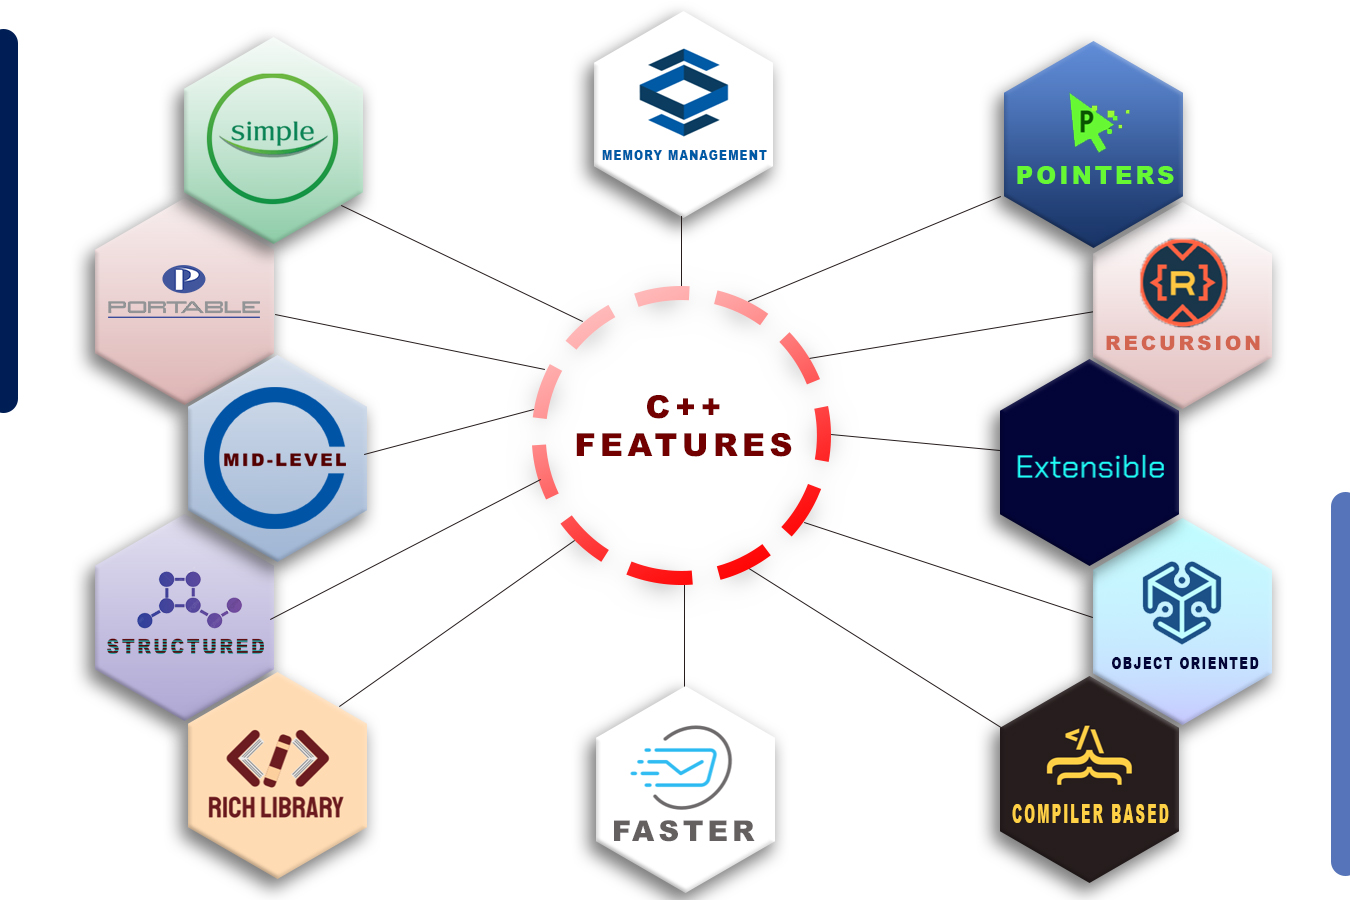
\includegraphics[scale=0.2]{Project_images/c++1.png}}; 
\end{tikzpicture}

\vspace{6cm}
\href{https://www.w3schools.com/cpp/cpp_oop.asp}{\textbf{C++ OOP}}

\end{frame}

%frame4

\begin{frame}
\frametitle{\textbf{Și pentru ce anume?}}

\vspace{-2.8cm}
\begin{enumerate}
  \item \textit{Toolkit special folosit pentru simularea detectorilor de radiație}
  \item \textit{Numeroase funcții și librării - flexibil și ușor de folosit.}
  \item \textit{Structură de dependență circulară între categorii.}
  \item \textit{Multiple modele tehnice de aplicații.}
\end{enumerate}

%exemple1 -HGPE
\begin{tikzpicture}[overlay, remember picture]
\node[anchor=center, 
      xshift=-3.5cm, 
      yshift=-2.5cm] 
     at (current page.center) 
     {\includegraphics[scale=0.18]{Project_images/HG.png}}; 
\end{tikzpicture}

%RealSim
\begin{tikzpicture}[overlay, remember picture]
\node[anchor=center, 
      xshift=-2cm, 
      yshift=0.3cm] 
     at (current page.center) 
     {\includegraphics[scale=0.18]{Project_images/logo-dark.png}}; 
\end{tikzpicture}

%exemple 2 -gamma det
\begin{tikzpicture}[overlay, remember picture]
\node[anchor=center, 
      xshift=2.6cm, 
      yshift=-2.1cm] 
     at (current page.center) 
     {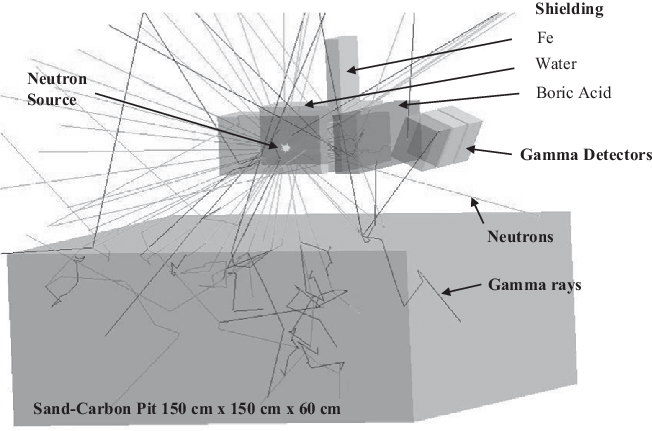
\includegraphics[scale=0.21]{Project_images/The-MC-simulation-model-Geant4-of-the-current-3-detector-unmodified-INS-system-for.png}}; 
\end{tikzpicture}

%exemple 3 -gears
\begin{tikzpicture}[overlay, remember picture]
\node[anchor=center, 
      xshift=4cm, 
      yshift=1cm] 
     at (current page.center) 
     {
\includegraphics[scale=0.2]{simulation.png}}; 
\end{tikzpicture}



\end{frame}



%%%%%%%%%%%%%%%%%%%%%%%%%%%%%%%%%%%%%%%%%%%%%%%%%%%%%%%%%%%%%%%%%%%%%%%%%%
%%%%%%%%%%%%%%%%%%%%%%%%%%%%%%%%%%%%%%%%%%%%%%%%%%%%%%%%%%%%%%%%%%%%%%%%

%sub sect 2
\subsection{Artă în Geant4- ce oferă?}

%fram2
\begin{frame}
\frametitle{\textbf{Structură de substructură;}}

%imag1
\begin{tikzpicture}[overlay, remember picture]
\node[anchor=center, 
      xshift=-3cm, 
      yshift=-0.5cm] 
     at (current page.center) 
     {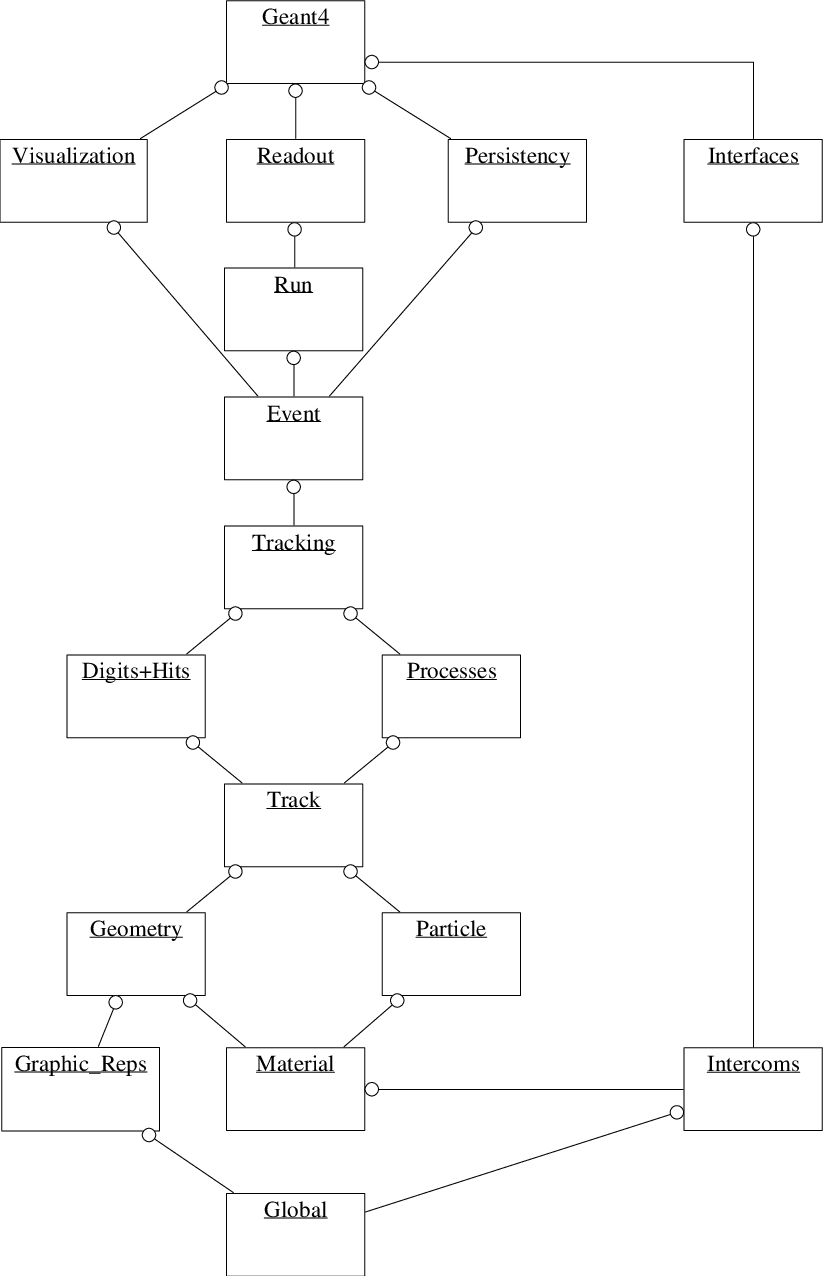
\includegraphics[scale=0.16]{Project_images/The-Top-Level-Category-Diagram-of-the-Geant4-toolkit-The-open-circle-on-the-joining.png}}; 
\end{tikzpicture}


%imag2
\begin{tikzpicture}[overlay, remember picture]
\node[anchor=center, 
      xshift=3cm, 
      yshift=-0.5cm] 
     at (current page.center) 
     {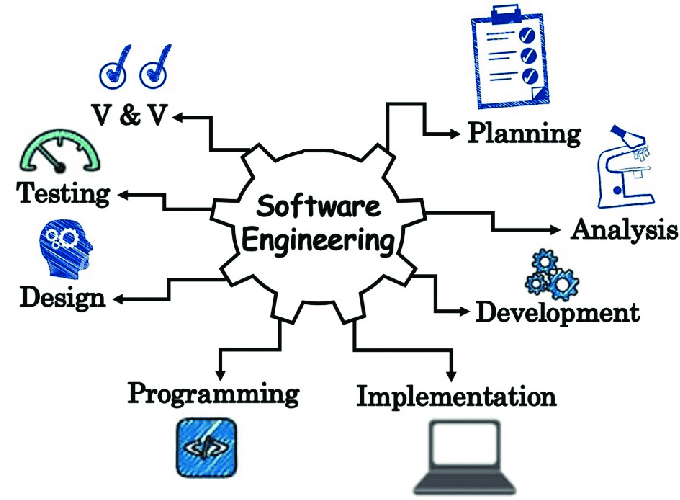
\includegraphics[scale=0.25]{Project_images/Soft.png}}; 
\end{tikzpicture}


\begin{tikzpicture}[overlay, remember picture]
\node[anchor=center, 
      xshift=3cm, 
      yshift=2cm] 
     at (current page.center) 
     {
\includegraphics[scale=0.18]{Project_images/ce519a43ebdf7ac48a98a03c6ad6eea013b68c46.png}}; 
\end{tikzpicture}

\end{frame}



%frame3

\begin{frame}
       \frametitle{\textbf{Features:}}


%continut
\vspace*{-0.9cm} %pozitionare relativ la top 

\textit{\textbf{Ce oferă GEANT4?}}

\begin{enumerate}

\color{blue}
\item[$\ast$] Geometry

\color{red}
\item[$\ast$] Tracking

\color{black}
\item[$\ast$] Detector Response

\color{green}
\item[$\ast$] Run management

\color{cyan}
\item[$\ast$] Visualisation

\end{enumerate}

%Window
\begin{tikzpicture}[overlay, remember picture]
\node[anchor=center, 
      xshift=2cm, 
      yshift=1cm] 
     at (current page.center) 
     {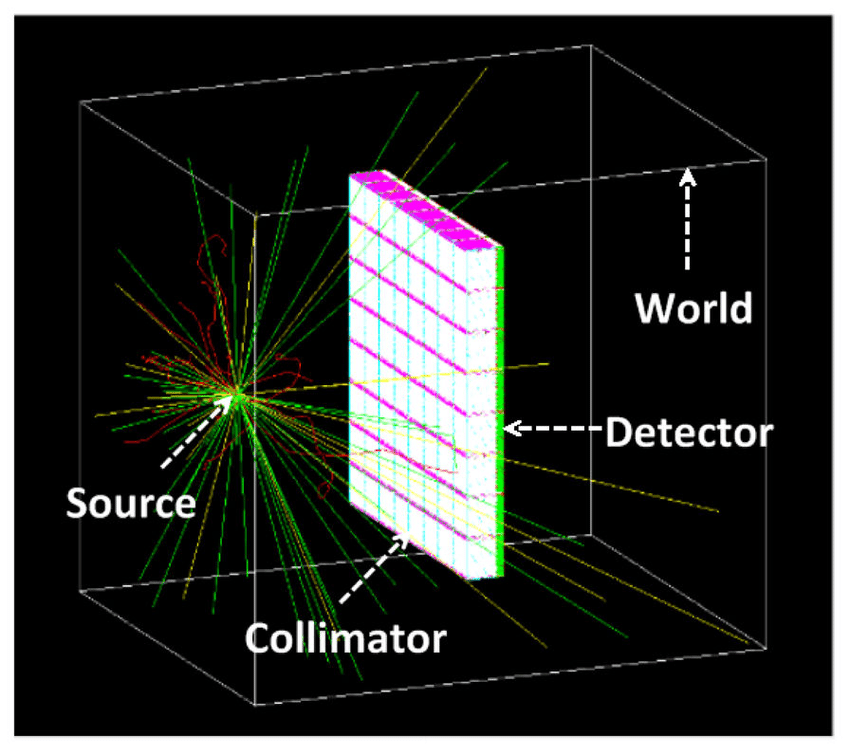
\includegraphics[scale=0.15, cfbox=blue 1pt 1pt]{Project_images/Comp.png}}; 
\end{tikzpicture}

%Ge TRacks det
\begin{tikzpicture}[overlay, remember picture]
\node[anchor=center, 
      xshift=2cm, 
      yshift=-2.5cm] 
     at (current page.center) 
     {\includegraphics[scale=0.2]{Project_images/tracksGe.png}}; 
\end{tikzpicture}

%imagine avantaje
\begin{tikzpicture}[overlay, remember picture]
\node[anchor=center, 
      xshift=-4cm, 
      yshift=-2.5cm] 
     at (current page.center) 
     {
\includegraphics[width=3.4cm,height=2.1cm]{Project_images/FUnctions.png}}; 
\end{tikzpicture}


\end{frame}

%another slide, ANOTHER IDEA
\begin{frame}{\textbf{INTERFACE:}}
    
\begin{tikzpicture}[overlay, remember picture]
\node[anchor=center, 
      xshift=0cm, 
      yshift=-0.5cm] 
     at (current page.center) 
     {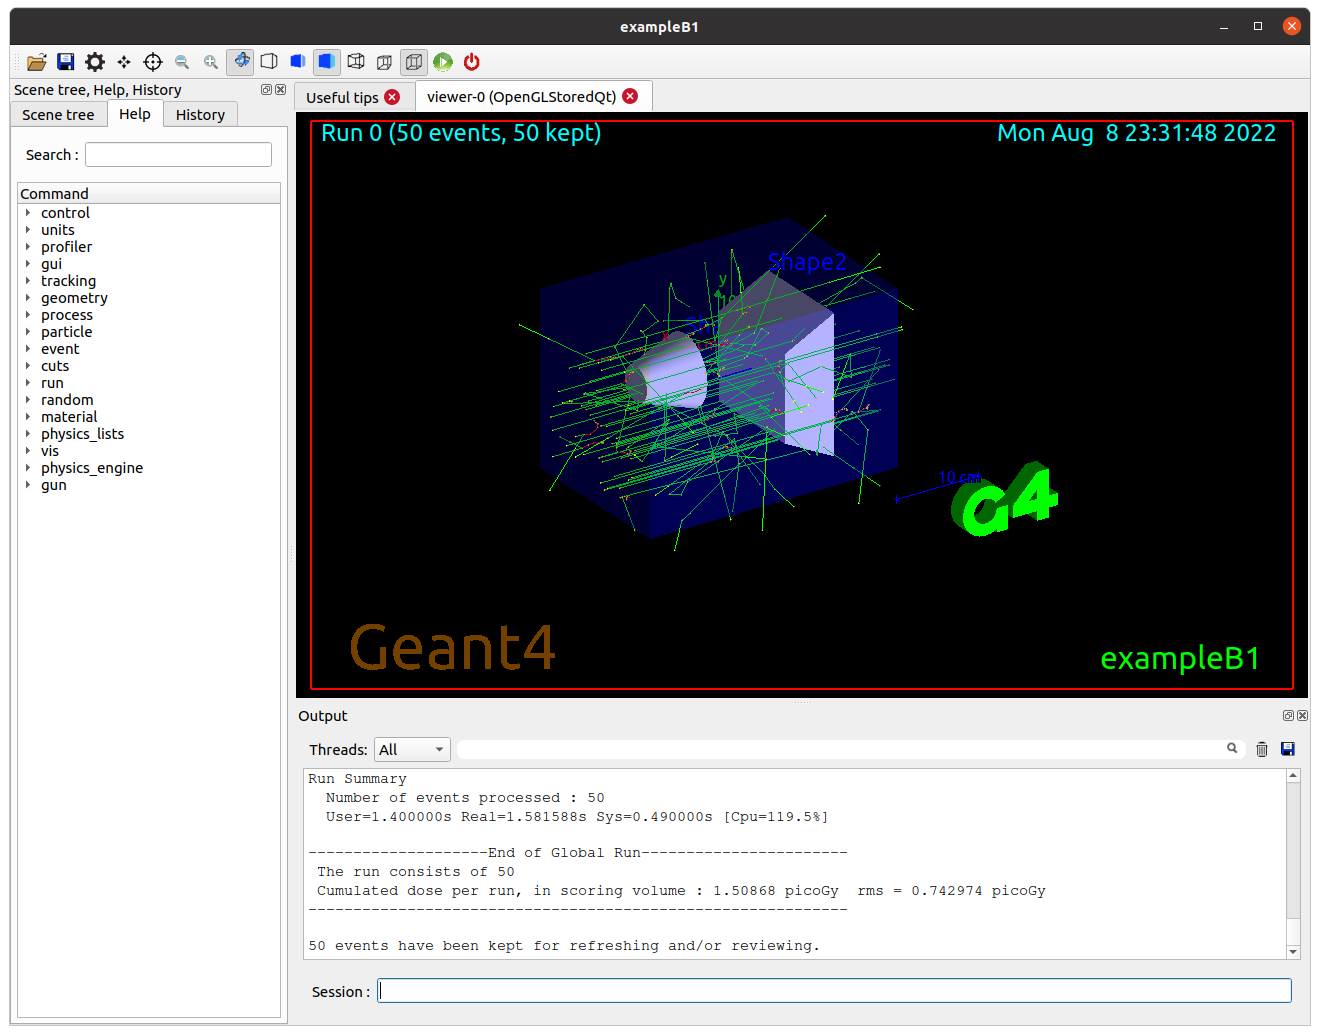
\includegraphics[width=10.5cm,height=7cm]{Project_images/INterface.png}}; 
\end{tikzpicture}
\end{frame}

%steps frm
\begin{frame}{Step1-Open(first... \href{https://www.youtube.com/watch?v=Lxb4WZyKeCE}{\textbf{Install?}})}

%imag1 - open the folder
\begin{tikzpicture}[overlay, remember picture]
\node[anchor=center, 
      xshift=-2cm, 
      yshift=0.5cm] 
     at (current page.center) 
     {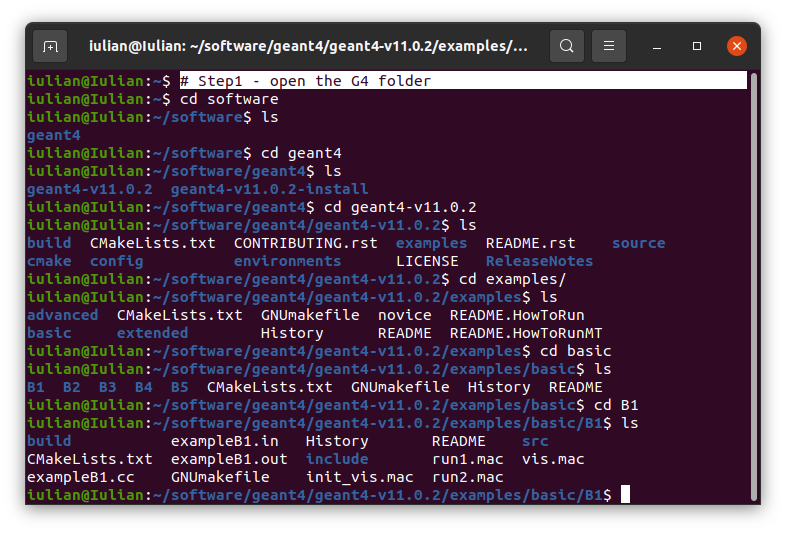
\includegraphics[scale=0.3]{Project_images/S1.png}}; 
\end{tikzpicture}

%imag2 - UBUNTU - setp1 - open the folder
\begin{tikzpicture}[overlay, remember picture]
\node[anchor=center, 
      xshift=4cm, 
      yshift=-1cm] 
     at (current page.center) 
     {
\includegraphics[scale=0.06]{Project_images/maxresdefault.jpg}}; 
\end{tikzpicture}

%imag3 - directories
\begin{tikzpicture}[overlay, remember picture]
\node[anchor=center, 
      xshift=4.1cm, 
      yshift=1.5cm] 
     at (current page.center) 
     {\includegraphics[scale=0.21]{Project_images/StrC++.png}}; 
\end{tikzpicture}

\vspace*{3.5cm} 
The Linux cd command offers several ways to navigate and change the working directory using the terminal window.


\end{frame}


%Step2- put
\begin{frame}{Step2-build, compile and run - "bcr"}
\begin{tikzpicture}[overlay, remember picture]

\node[anchor=center, 
      xshift=0cm, 
      yshift=-0.5cm] 
     at (current page.center) 
     {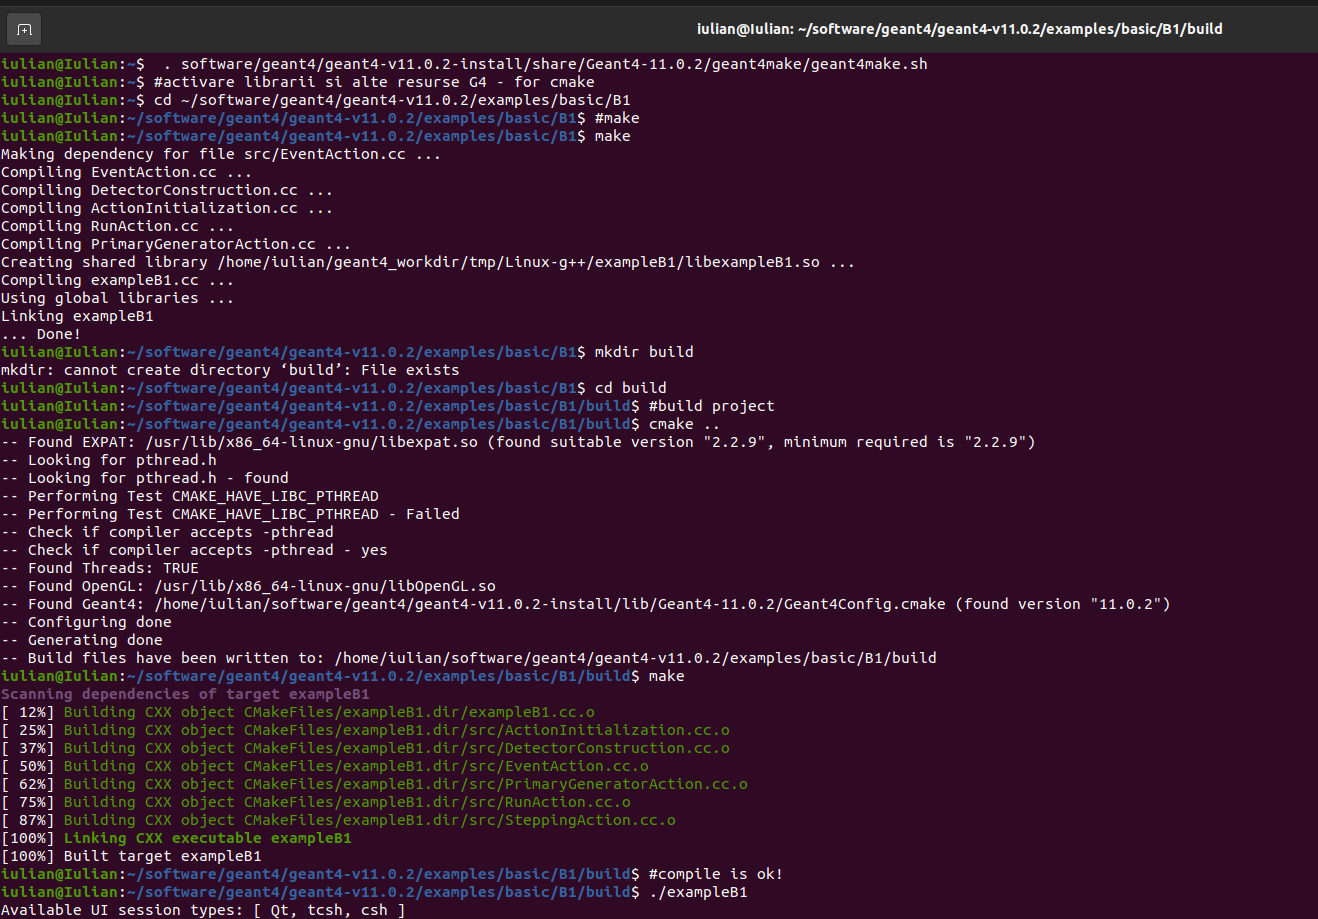
\includegraphics[scale=0.22, cfbox = blue 1pt 1pt]{Project_images/Step2.png}}; 
\end{tikzpicture}

\end{frame}

%Step2- put
\begin{frame}{Objects- examples}
\begin{tikzpicture}[overlay, remember picture]

\node[anchor=center, 
      xshift=-1cm, 
      yshift=-0.5cm] 
     at (current page.center) 
     {\includegraphics[scale=0.3]{Project_images/ClassInit.png}}; 
\end{tikzpicture}

\end{frame}



%NOT final - rest for test
\begin{frame}{\textbf{Detector simulation parts:}}

%parts1 - marker
\begin{tikzpicture}[overlay, remember picture]
\node[anchor=center, 
      xshift=-3cm, 
      yshift=1.2cm] 
     at (current page.center) 
     {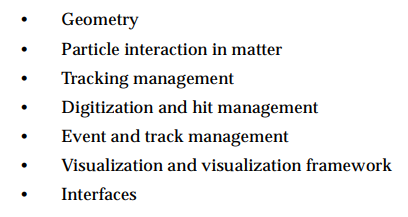
\includegraphics[scale=0.7]{Project_images/DetectorParts.png}}; 
\end{tikzpicture}

%parts2 - blocks
\begin{tikzpicture}[overlay, remember picture]
\node[anchor=center, 
      xshift=3cm, 
      yshift=-1.8cm] 
     at (current page.center) 
     {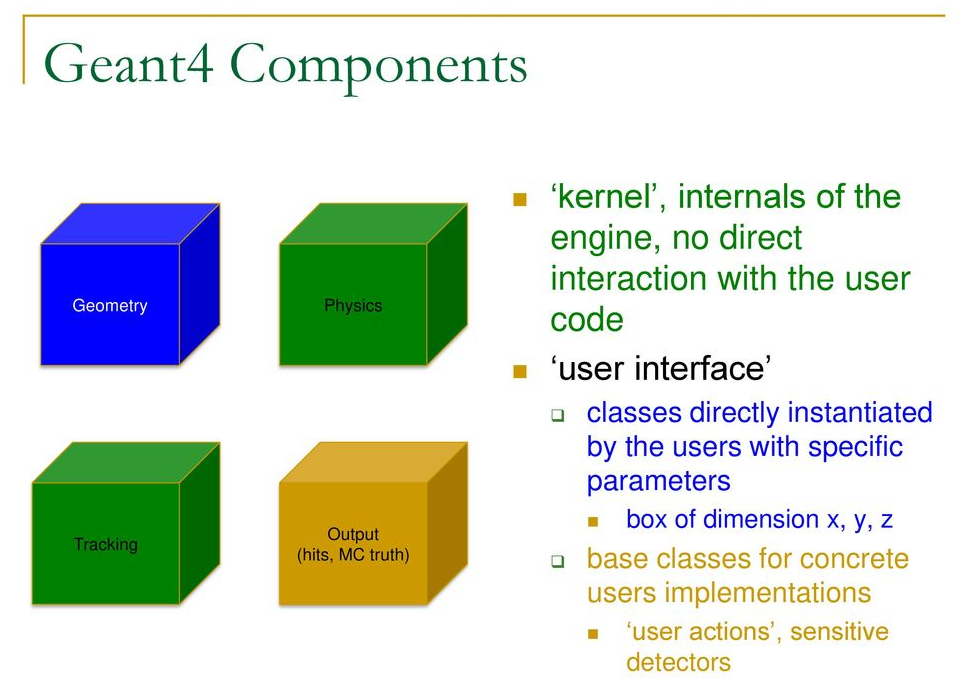
\includegraphics[scale=0.3]{Project_images/G4Comp..png}}; 
\end{tikzpicture}


%parts3 - OOP
\begin{tikzpicture}[overlay, remember picture]
\node[anchor=center, 
      xshift=2.5cm, 
      yshift=1.8cm] 
     at (current page.center) 
     {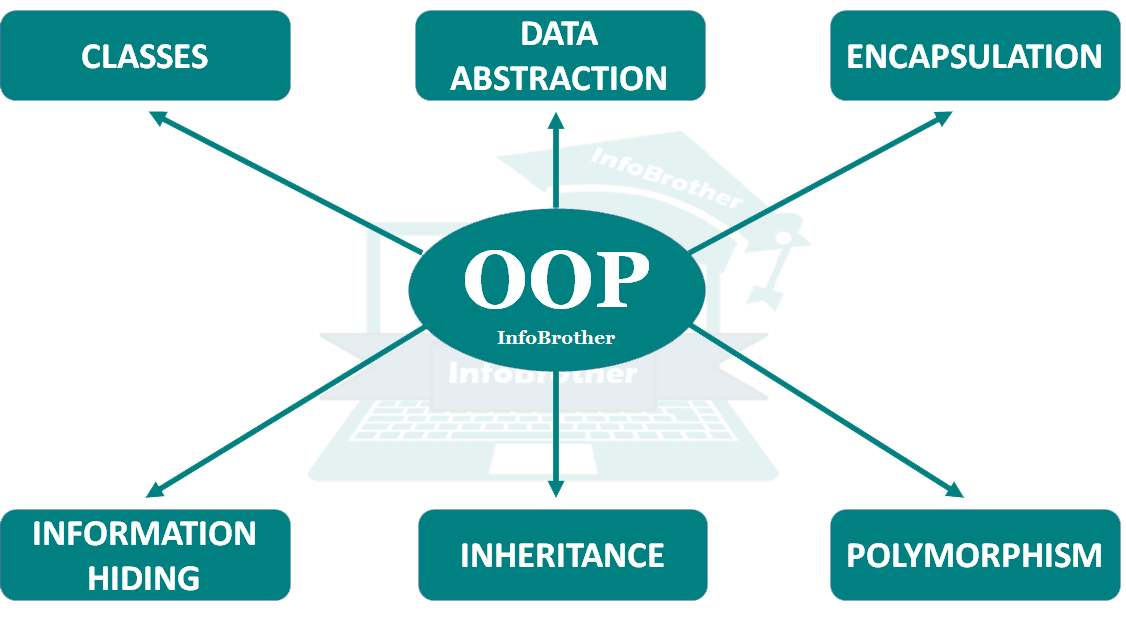
\includegraphics[scale=0.1, cfbox = purple 1pt 1pt]{Project_images/Program.png}}; 
\end{tikzpicture}


%parts4 - monteCarlo
\begin{tikzpicture}[overlay, remember picture]
\node[anchor=center, 
      xshift=-3.5cm, 
      yshift=-2.0cm] 
     at (current page.center) 
     {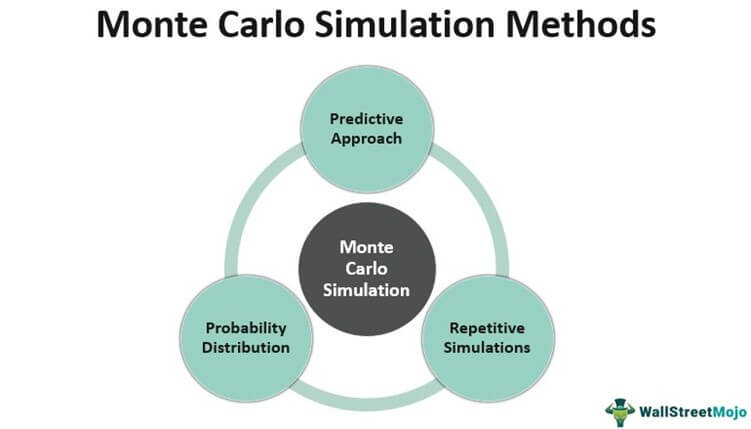
\includegraphics[scale=0.22]{Project_images/Monte-Carlo-Simulation-methods.png}}; 
\end{tikzpicture}

\end{frame}



%supl. frame
\begin{frame}{\textbf{A Simple Diagram:}}

%contextual diagram
\begin{tikzpicture}[overlay, remember picture]
\node[anchor=center, 
      xshift=-2cm, 
      yshift=-0.5cm] 
     at (current page.center) 
     {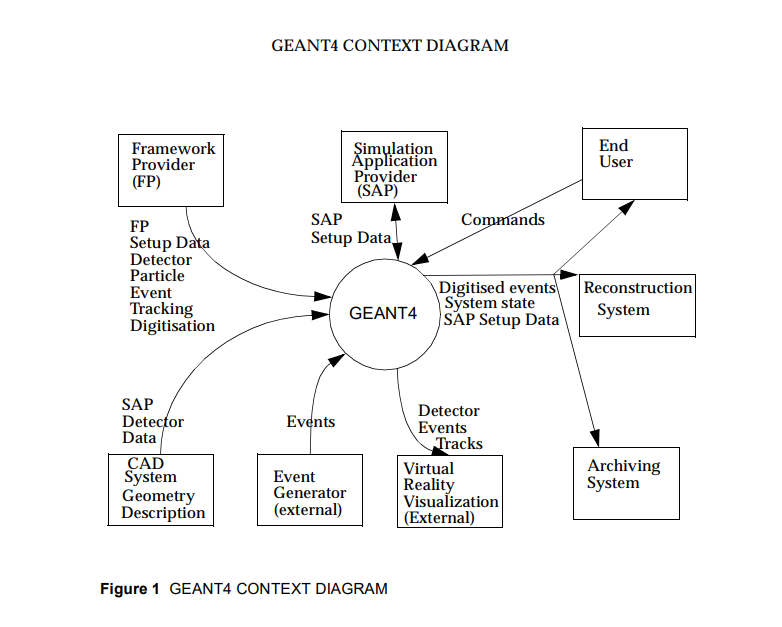
\includegraphics[scale=0.55]{Project_images/Coxtextual Diagram.png}}; 
\end{tikzpicture}

%image det. diag.
\begin{tikzpicture}[overlay, remember picture]
\node[anchor=center, 
      xshift=4cm, 
      yshift=-0.5cm] 
     at (current page.center) 
     {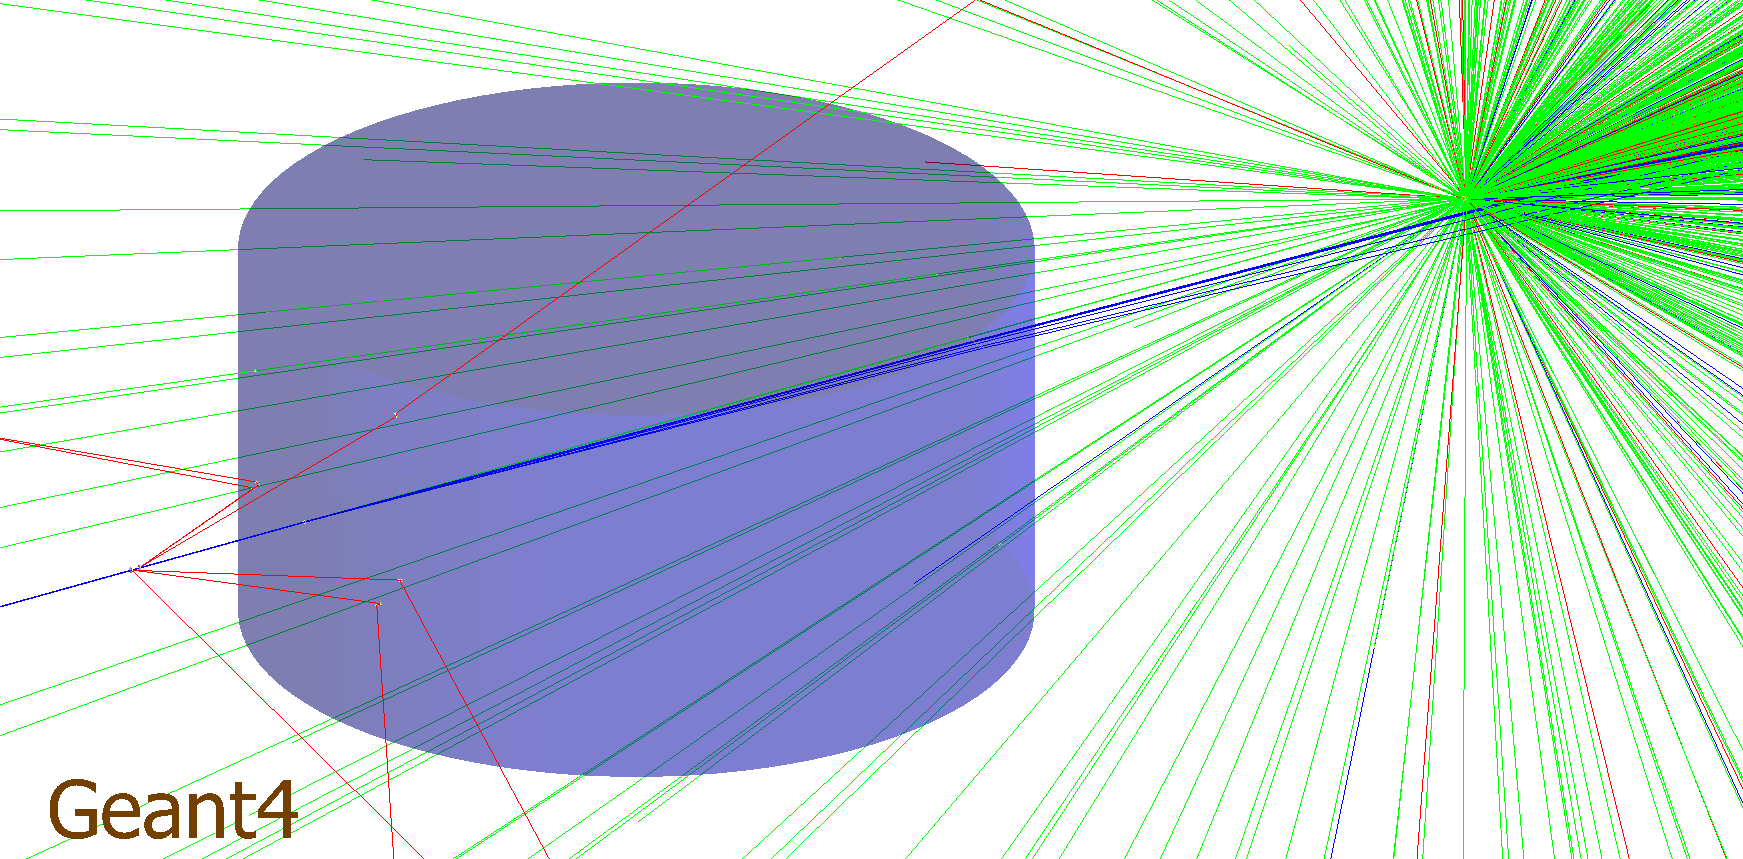
\includegraphics[scale=0.1, angle=90, cfbox=black 1pt 1pt]{Project_images/b21c4c5181c0773d36c05760c0216ae050c306a7.png}}; 
\end{tikzpicture}

%image det. diag.
\begin{tikzpicture}[overlay, remember picture]
\node[anchor=center, 
      xshift=-5cm, 
      yshift=2.5cm] 
     at (current page.center) 
     {
\includegraphics[scale=0.05]{Project_images/custo.png}}; 
\end{tikzpicture}
    
\end{frame}

%HEP EXPERIMENT
\begin{frame}{\textbf{CONFIGURATION:}}

%picture1 HEP
\begin{tikzpicture}[overlay, remember picture]
\node[anchor=center, 
      xshift=0cm, 
      yshift=-0.1cm] 
     at (current page.center) 
     {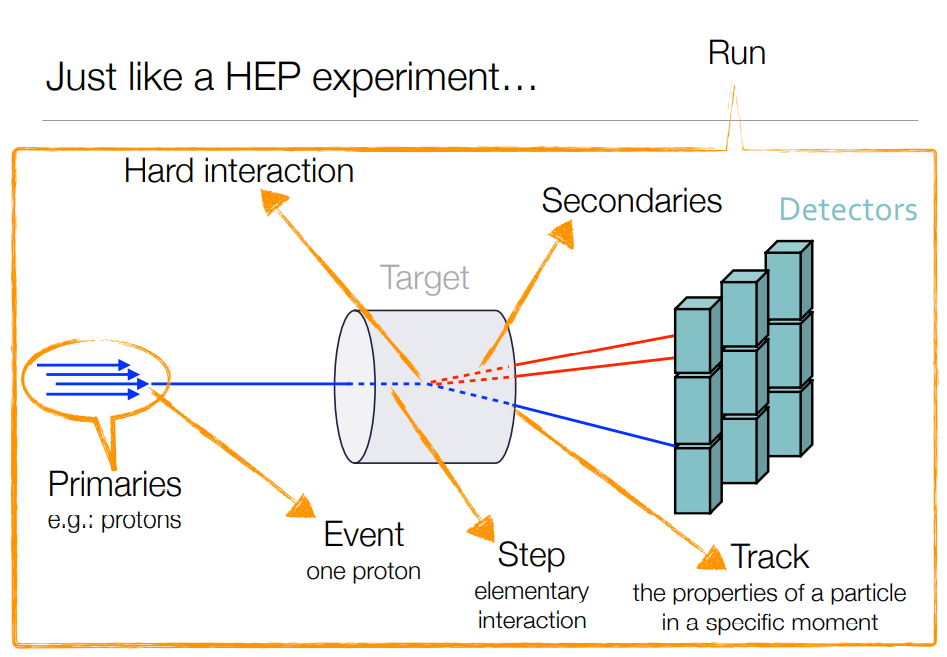
\includegraphics[scale=0.5]{Project_images/HEP.png}}; 
\end{tikzpicture}

%picture2 reality
\begin{tikzpicture}[overlay, remember picture]
\node[anchor=center, 
      xshift=-5.5cm, 
      yshift=2.5cm] 
     at (current page.center) 
     {
\includegraphics[scale=0.2,angle=45]{real.png}}; 
\end{tikzpicture}

%fantasy = picture3
\begin{tikzpicture}[overlay, remember picture]
\node[anchor=center, 
      xshift=5.5cm, 
      yshift=2.5cm] 
     at (current page.center) 
     {
\includegraphics[scale=0.25,angle=45]{Project_images/fan.png}}; 
\end{tikzpicture}


\end{frame}


%new frame - ORGANIGRAMA
\begin{frame}{OR... CE?}

%DIAGRAM
\begin{tikzpicture}[overlay, remember picture]
\node[anchor=center, 
      xshift=-2cm, 
      yshift=0cm] 
     at (current page.center) 
     {\includegraphics[scale=0.25]{Project_images/Flow.png}}; 
\end{tikzpicture}

%JARGON - img2
\begin{tikzpicture}[overlay, remember picture]
\node[anchor=center, 
      xshift=4cm, 
      yshift=-2cm] 
     at (current page.center) 
     {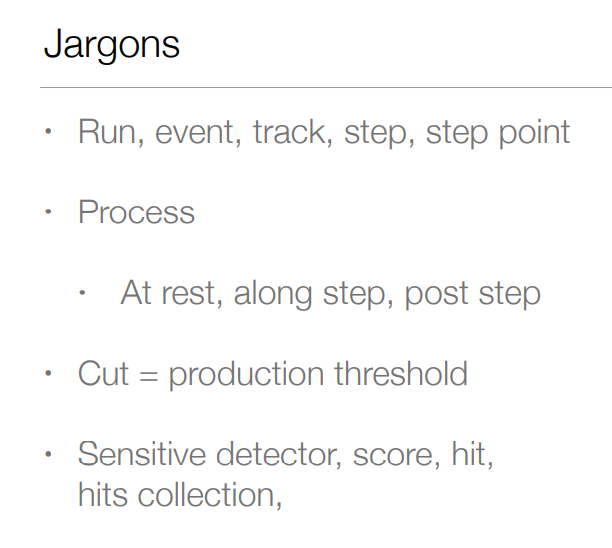
\includegraphics[scale=0.3]{Project_images/G4Jargon.png}}; 
\end{tikzpicture}

%ImagAlgCircle- imag3
\begin{tikzpicture}[overlay, remember picture]
\node[anchor=center, 
      xshift=4cm, 
      yshift=1cm] 
     at (current page.center) 
     {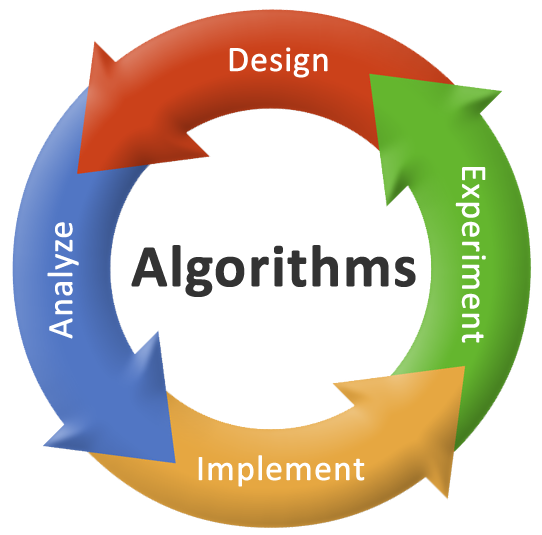
\includegraphics[scale=0.14]{Project_images/cs161logo.png}};
\end{tikzpicture}

%EVENT- imag4
\begin{tikzpicture}[overlay, remember picture]
\node[anchor=center, 
      xshift=-3.0cm, 
      yshift=-3.5cm] 
     at (current page.center) 
     {
\includegraphics[scale=0.18]{BE_events.png}};
\end{tikzpicture}

\end{frame}

%%%%%%%%%%%%%%%%%%%%%%%%%%%%%%%%%%%%%%%%%%%%%%%%%%%%%%%%%%%%%%%%%%%

%clase generale

\begin{frame}{\textbf{Clase.} }

%user classes
\begin{tikzpicture}[overlay, remember picture]
\node[anchor=center, 
      xshift=-3.5cm, 
      yshift=-0.5cm] 
     at (current page.center) 
  {\includegraphics[scale=0.3]{Project_images/Screenshot from 2022-08-10 11-33-55.png}};
\end{tikzpicture}

%class structure
\begin{tikzpicture}[overlay, remember picture]
\node[anchor=center, 
      xshift=3cm, 
      yshift=1.5cm] 
     at (current page.center) 
  {\includegraphics[scale=0.3]{Project_images/classStructure.png}};
\end{tikzpicture}

%optional 
\begin{tikzpicture}[overlay, remember picture]
\node[anchor=center, 
      xshift=3.0cm, 
      yshift=-1.9cm] 
     at (current page.center) 
  {\includegraphics[scale=0.3]{Project_images/otional.png}};
\end{tikzpicture}


\end{frame}


%%%%%%%%%%%%%%%%%%%%%%%%%%%%%%%%%%%%%%%%%%%%%%%%%%%%%%%%%%%%%%%%%%%
%clase optionale
\begin{frame}{\textbf{Clase optionale.} }

\begin{tikzpicture}[overlay, remember picture]
\node[anchor=center, 
      xshift=0cm, 
      yshift=-0.5cm] 
     at (current page.center) 
     {\includegraphics[scale=0.3]{Project_images/optional1.png}};
\end{tikzpicture}


\end{frame}


%%%%%%%%%%%%%%%%%%%%%%%%%%%%%%%%%%%%%%%%%%%%%%%%%%%%%%%%%%%%%%%%%%%
%class map(harta)
\begin{frame}{\textbf{O hartă... mentală sau reală?} }

\begin{tikzpicture}[overlay, remember picture]
\node[anchor=center, 
      xshift=0cm, 
      yshift=-0.5cm] 
     at (current page.center) 
     {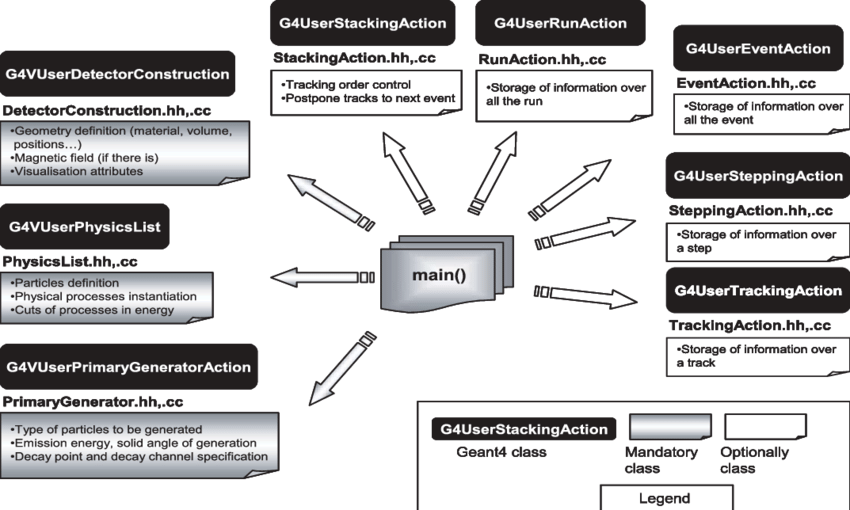
\includegraphics[scale=0.35]{Project_images/Mandatory-and-some-optionally-classes-needed-by-a-GEANT4-based-application.png}};
\end{tikzpicture}


\end{frame}


%ce avem de facut1
\begin{frame}{\textbf{Ce avem de facut?} }

\begin{tikzpicture}[overlay, remember picture]
\node[anchor=center, 
      xshift=0cm, 
      yshift=0cm] 
     at (current page.center) 
     {\includegraphics[scale=0.4]{Project_images/1.png}};
\end{tikzpicture}
\end{frame}

%ce avem de facut2
\begin{frame}{\textbf{Ce avem de facut?} }

\begin{tikzpicture}[overlay, remember picture]
\node[anchor=center, 
      xshift=0cm, 
      yshift=0cm] 
     at (current page.center) 
     {\includegraphics[scale=0.4]{Project_images/2.png}};
\end{tikzpicture}
\end{frame}

%ce avem de facut3
\begin{frame}{\textbf{Ce avem de făcut?} }

\begin{tikzpicture}[overlay, remember picture]
\node[anchor=center, 
      xshift=0cm, 
      yshift=-0.5cm] 
     at (current page.center) 
     {\includegraphics[scale=0.4]{Project_images/3.png}};
\end{tikzpicture}
\end{frame}

%ce avem de facut4
\begin{frame}{\textbf{Ce avem de făcut?} }

\begin{tikzpicture}[overlay, remember picture]
\node[anchor=center, 
      xshift=0cm, 
      yshift=-0.5cm] 
     at (current page.center) 
     {\includegraphics[scale=0.4]{Project_images/4.png}};
\end{tikzpicture}
\end{frame}

%ce avem de facut5
\begin{frame}{\textbf{Ce avem de făcut?} }

\begin{tikzpicture}[overlay, remember picture]
\node[anchor=center, 
      xshift=0cm, 
      yshift=-0.5cm] 
     at (current page.center) 
     {\includegraphics[scale=0.4]{Project_images/5.png}};
\end{tikzpicture}
\end{frame}

%ce avem de facut6
\begin{frame}{\textbf{Ce avem de facut?} }

\begin{tikzpicture}[overlay, remember picture]
\node[anchor=center, 
      xshift=0cm, 
      yshift=-0.5cm] 
     at (current page.center) 
     {\includegraphics[scale=0.4]{Project_images/6.png}};
\end{tikzpicture}


\end{frame}

%%%%%%%%%%%%%%%%%%%%%%%%%%%%%%%%%%%%%%%%%%%%%%%%%%%%%%%%%%%%
%frame for MonteCarlo
\begin{frame}{\href{https://gfycat.com/bewitchedviciousaltiplanochinchillamouse-irrational-numbers-approximation}{\textbf{Monte Carlo?}}}

\vspace{-3cm}
\begin{enumerate}
  \item[I)] \textbf{To determine the experimental setup.}
  \item[II)] \textbf{Compare the results(experimental vs simulated).}
  \item[III)] \textbf{Correct or optimize the results.}
  \item[IV)] \textbf{More...}


\end{enumerate}

%picture1-pi estimation
\begin{tikzpicture}[overlay, remember picture]
\node[anchor=center, 
      xshift=2.5cm, 
      yshift=-1cm] 
     at (current page.center) 
     {\includegraphics[scale=0.35]{Project_images/SemiCarloMehtodPi.png}};
\end{tikzpicture}

%picture2-MonteCarlo alg.
\begin{tikzpicture}[overlay, remember picture]
\node[anchor=center, 
      xshift=-3.5cm, 
      yshift=-1.5cm] 
     at (current page.center) 
     {\includegraphics[scale=0.25]{Project_images/1_GAsEOl5w9370HpVmG7We_A.png}};
\end{tikzpicture}




\end{frame}
%------------------------------------------------

%%%%%%%%%%%%%%%%%%%%%%%%%%%%%%%%%%%%%%%%%%%%%%%%%%%%%%%%%%%%%%%%%%%%%%%%%%%%%%%%%%%
%%%%%%%%%%%%%%%%%%%%%%%%%%%%%%%%%%%%%%%%%%%%%%%%%%%%%%%%%%%%%%%%%%%%%%%%%%%%%%%%%%%


%SECTION2
\section{Un mic proiect.}
%------------------------------------------------

%sect 1
\subsection{Despre?}

\begin{frame}{\textbf{Ce am plăsmuit?}}

\vspace{-2cm}

\begin{itemize}   
  \item Simularea unui detector de radiație Cherenkov!
  \item O matrice/grid(100x100) de detectori 3D, fotosensibili(voxeli)!
  \item Simularea + rularea evenimentului fizic!
\end{itemize}


%output- imag1
\begin{tikzpicture}[overlay, remember picture]
\node[anchor=center, 
      xshift=-4.5cm, 
      yshift=0.5cm] 
     at (current page.center) 
     {\includegraphics[scale=0.06]{Project_images/output-vector-logo.png}};
\end{tikzpicture}


%Simulation- imag2
\begin{tikzpicture}[overlay, remember picture]
\node[anchor=center, 
      xshift=3cm, 
      yshift=-2cm] 
     at (current page.center) 
     {\includegraphics[scale=0.5]{Project_images/ringPattern.png}};
\end{tikzpicture}


%Simulation Hits Impact- imag3
\begin{tikzpicture}[overlay, remember picture]
\node[anchor=center, 
      xshift=-2.5cm, 
      yshift=-2cm] 
     at (current page.center) 
     {\includegraphics[scale=0.3]{Project_images/P1.png}};
\end{tikzpicture}


%Simulation Hits Impact- imag3
\begin{tikzpicture}[overlay, remember picture]
\node[anchor=center, 
      xshift=3.0cm, 
      yshift=0.5cm] 
     at (current page.center) 
     {\includegraphics[scale=0.3]{Project_images/LOGOcerenkov-01-removebg-preview.png}};
\end{tikzpicture}


\end{frame}

%sect 2
\subsection{Cod de diagramă sau diagramă de cod?}


\begin{frame}{\textbf{WEB?}}

%canvas web - imag1
\begin{tikzpicture}[overlay, remember picture]
\node[anchor=center, 
      xshift=1cm, 
      yshift=0cm] 
     at (current page.center) 
     {\includegraphics[scale=0.5, cfbox = orange 1pt 1pt]{Project_images/Diag.png}};
\end{tikzpicture}

%imag2 - list
\begin{tikzpicture}[overlay, remember picture]
\node[anchor=center, 
      xshift=-5.3cm, 
      yshift=-1.0cm] 
     at (current page.center) 
     {\includegraphics[scale=0.5, cfbox = cyan 1pt 1pt]{Project_images/all.png}};
\end{tikzpicture}

%corelation- imag3
\begin{tikzpicture}[overlay, remember picture]
\node[anchor=center, 
      xshift=-2cm, 
      yshift=-2.5cm] 
     at (current page.center) 
     {\includegraphics[scale=0.1]{connection-a-division-of-elettromedia-vector-logo.png}};
\end{tikzpicture}

%code
\vspace{-6cm}
\href{https://github.com/Pixel20000/Geant4_FirstProject}{\textbf{-MyCode-}}

\end{frame}




%%%%%%%%%%%%%%%%%%%%%%%%%%%%%%%%%%%%%%%%%%%%%%%%%%%%%%%%%%%%%%%%

\section{Concluzii dar nu iluzii!}
\subsection{De folos?}

%final frame
\begin{frame}{\textbf{Need... for?}}

%imag1 apps
\begin{tikzpicture}[overlay, remember picture]
\node[anchor=center, 
      xshift=0cm, 
      yshift=1.2cm] 
     at (current page.center) 
     {\includegraphics[scale=0.37]{Project_images/aplicatiiUTILE.png}};
\end{tikzpicture}

%imag2 apps
\begin{tikzpicture}[overlay, remember picture]
\node[anchor=center, 
      xshift=-4.5cm, 
      yshift=-2.1cm] 
     at (current page.center) 
     {\includegraphics[scale=0.3]{Project_images/aplicatie1.png}};
\end{tikzpicture}


%imag3 detectorParts
\begin{tikzpicture}[overlay, remember picture]
\node[anchor=center, 
      xshift=2.6cm, 
      yshift=-2.2cm] 
     at (current page.center) 
     {\includegraphics[scale=0.7]{Project_images/1-s2.0-S0168900220302552-gr1.jpg}};
\end{tikzpicture}

%imag4 importance
\begin{tikzpicture}[overlay, remember picture]
\node[anchor=center, 
      xshift=-1.5cm, 
      yshift=-2cm] 
     at (current page.center) 
     {\includegraphics[scale=0.3]{Project_images/important-information-sign-icon-logo-important-information-sign-icon-logo-white-background-139651901.jpg}};
\end{tikzpicture}


\vspace{5cm}
\href{https://geant4.web.cern.ch/sites/default/files/geant4/reports/pictures/fullsize/poster-phys-final.pdf}{\textbf{UTIL LA CE?}}


\end{frame}


\begin{frame}{Alte surse:}
\vspace{0cm}

\begin{enumerate}

  \item[$\blacksquare$] \href{https://cds.cern.ch/record/491492/files/p107.pdf}{Prezentare1}

  \item[$\blacksquare$] \href{https://geant4.web.cern.ch/sites/default/files/geant4/support/training/CSC2000/CSCG4.pdf}{Prezentare2}

  \item[$\blacksquare$] \href{https://www.mn.uio.no/fysikk/english/research/about/infrastructure/ocl/nuclear-physics-research/presentations-at-group-meetings/geant4-introduction.pdf}{Prezentare3}

  \item[$\blacksquare$] \href{https://indico.cern.ch/event/75452/contributions/2089769/attachments/1049574/1496250/ExtractingInfoPart1.pdf}{Prezentare4}

  \item[$\blacksquare$] \href{https://indico.bnl.gov/event/12272/contributions/51347/attachments/35565/58063/Geant4_Kernel2.pdf}{Prezentare5}

  \item[$\blacksquare$] \href{https://www.ge.infn.it/geant4/training/pisa_jan2006/introduction.ppt}{Prezentare6}

  \item[$\blacksquare$] \href{http://geant4.in2p3.fr/2005/Workshop/ShortCourse/session1/J.Apostolakis.pdf}{Prezentare7}

  \item[$\blacksquare$] \href{ http://geant4.in2p3.fr/2005/Workshop/ShortCourse/session1/J.Apostolakis.pdf}{Prezentare8}

  \item[$\blacksquare$] \href{ 
  https://indico.tifr.res.in/indico/getFile.py/access?contribId=29&resId=1&materialId=slides&confId=5309}{Prezentare9}

  \item[$\blacksquare$] \href{  https://geant4.web.cern.ch/content/presentations
}{Prezentare10}

%aero space apps
\begin{tikzpicture}[overlay, remember picture]
\node[anchor=center, 
      xshift=2cm, 
      yshift=0cm] 
     at (current page.center) 
     {\includegraphics[scale=0.2]{Project_images/spatialApp.png}};
\end{tikzpicture}

\begin{tikzpicture}[overlay, remember picture]
\node[anchor=center, 
      xshift=2cm, 
      yshift=-3cm] 
     at (current page.center) 
     {\includegraphics[scale=0.2]{Project_images/apps.png}};
\end{tikzpicture}
 
\end{enumerate}


\end{frame}


\subsection{Un nou început tocmai început.}



%-------------------------------------------------------------%
%-------------------------------------------------------------%
%                                                             %
%                    The Last Page                            %
%                                                             %
%-------------------------------------------------------------%
%-------------------------------------------------------------%
%-------------------------------------------------------------%

\begin{frame}
\Huge{\centerline{\textcolor{red}{\textit{\textbf{Thank you!!!}}}}}
\huge{\centerline{\textcolor{green}{Questions?}}}


\normalsize{\centerline{Pixeliuli@yahoo.com}}

%CERN LOGO
\begin{tikzpicture}[overlay, remember picture]
\node[anchor=center, 
      xshift=-4.5cm, 
      yshift=3cm] 
     at (current page.center) 
     {\includegraphics[scale=0.05]{Project_images/cern.jpg}};
\end{tikzpicture}


%CERN CAD import
\begin{tikzpicture}[overlay, remember picture]
\node[anchor=center, 
      xshift=-3cm, 
      yshift=-2cm] 
     at (current page.center) 
     {\includegraphics[scale=0.4]{Project_images/CAD.png}};
\end{tikzpicture}

%Det
\begin{tikzpicture}[overlay, remember picture]
\node[anchor=center, 
      xshift=3cm, 
      yshift=-2cm] 
     at (current page.center) 
     {\includegraphics[scale=0.25]{Project_images/efi.png}};
\end{tikzpicture}

%GammaRaysAir
\begin{tikzpicture}[overlay, remember picture]
\node[anchor=center, 
      xshift=4.5cm, 
      yshift=3cm] 
     at (current page.center) 
     {\includegraphics[scale=0.25]{Project_images/ginair.png}};
\end{tikzpicture}

\end{frame}

%----------------------------------------------------------------------------------------



\begin{frame}{Final Destination!}
 
 \begin{tikzpicture}
    \foreach \i in {1,...,80} {
      \pgfmathparse{rnd}
      \definecolor{MyColor}{hsb}{\pgfmathresult,1,1}
      \pgfmathparse{3.0*rnd+1.0}
      \node[text=MyColor] at (10*rnd,6*rnd) {\scalebox{\pgfmathresult}{?}};
    };
  \end{tikzpicture}

\end{frame}

\end{document} 